% ============================================================================
% sections/sec3_methodology.tex
% ============================================================================
\section{Methodology and Framework}
\label{sec:methodology}

\subsection{System Architecture}
\label{sec:architecture}

OmniGuard-RAG is a four-ring, defense-in-depth pipeline. Every ring is a
direct, traceable response to one specific, paper-documented gap
identified in \Cref{sec:literature}: Ring~0 answers PIDP's query-path
attack, Ring~1 answers ordinary and PIDP-style corpus poisoning, Ring~2
answers TriShieldRAG's ``false consensus'' failure mode, and Ring~3
answers RAGuard's own stated leave-one-out collusion blind spot. A
persistent Dynamic Trust Store sits alongside the four rings rather than
inside any one of them, carrying evidence about individual documents
across queries within a session --- a capability none of the four rings
has on its own, since each evaluates a single query's retrieved context
in isolation.

\begin{figure}[htbp]
\centering
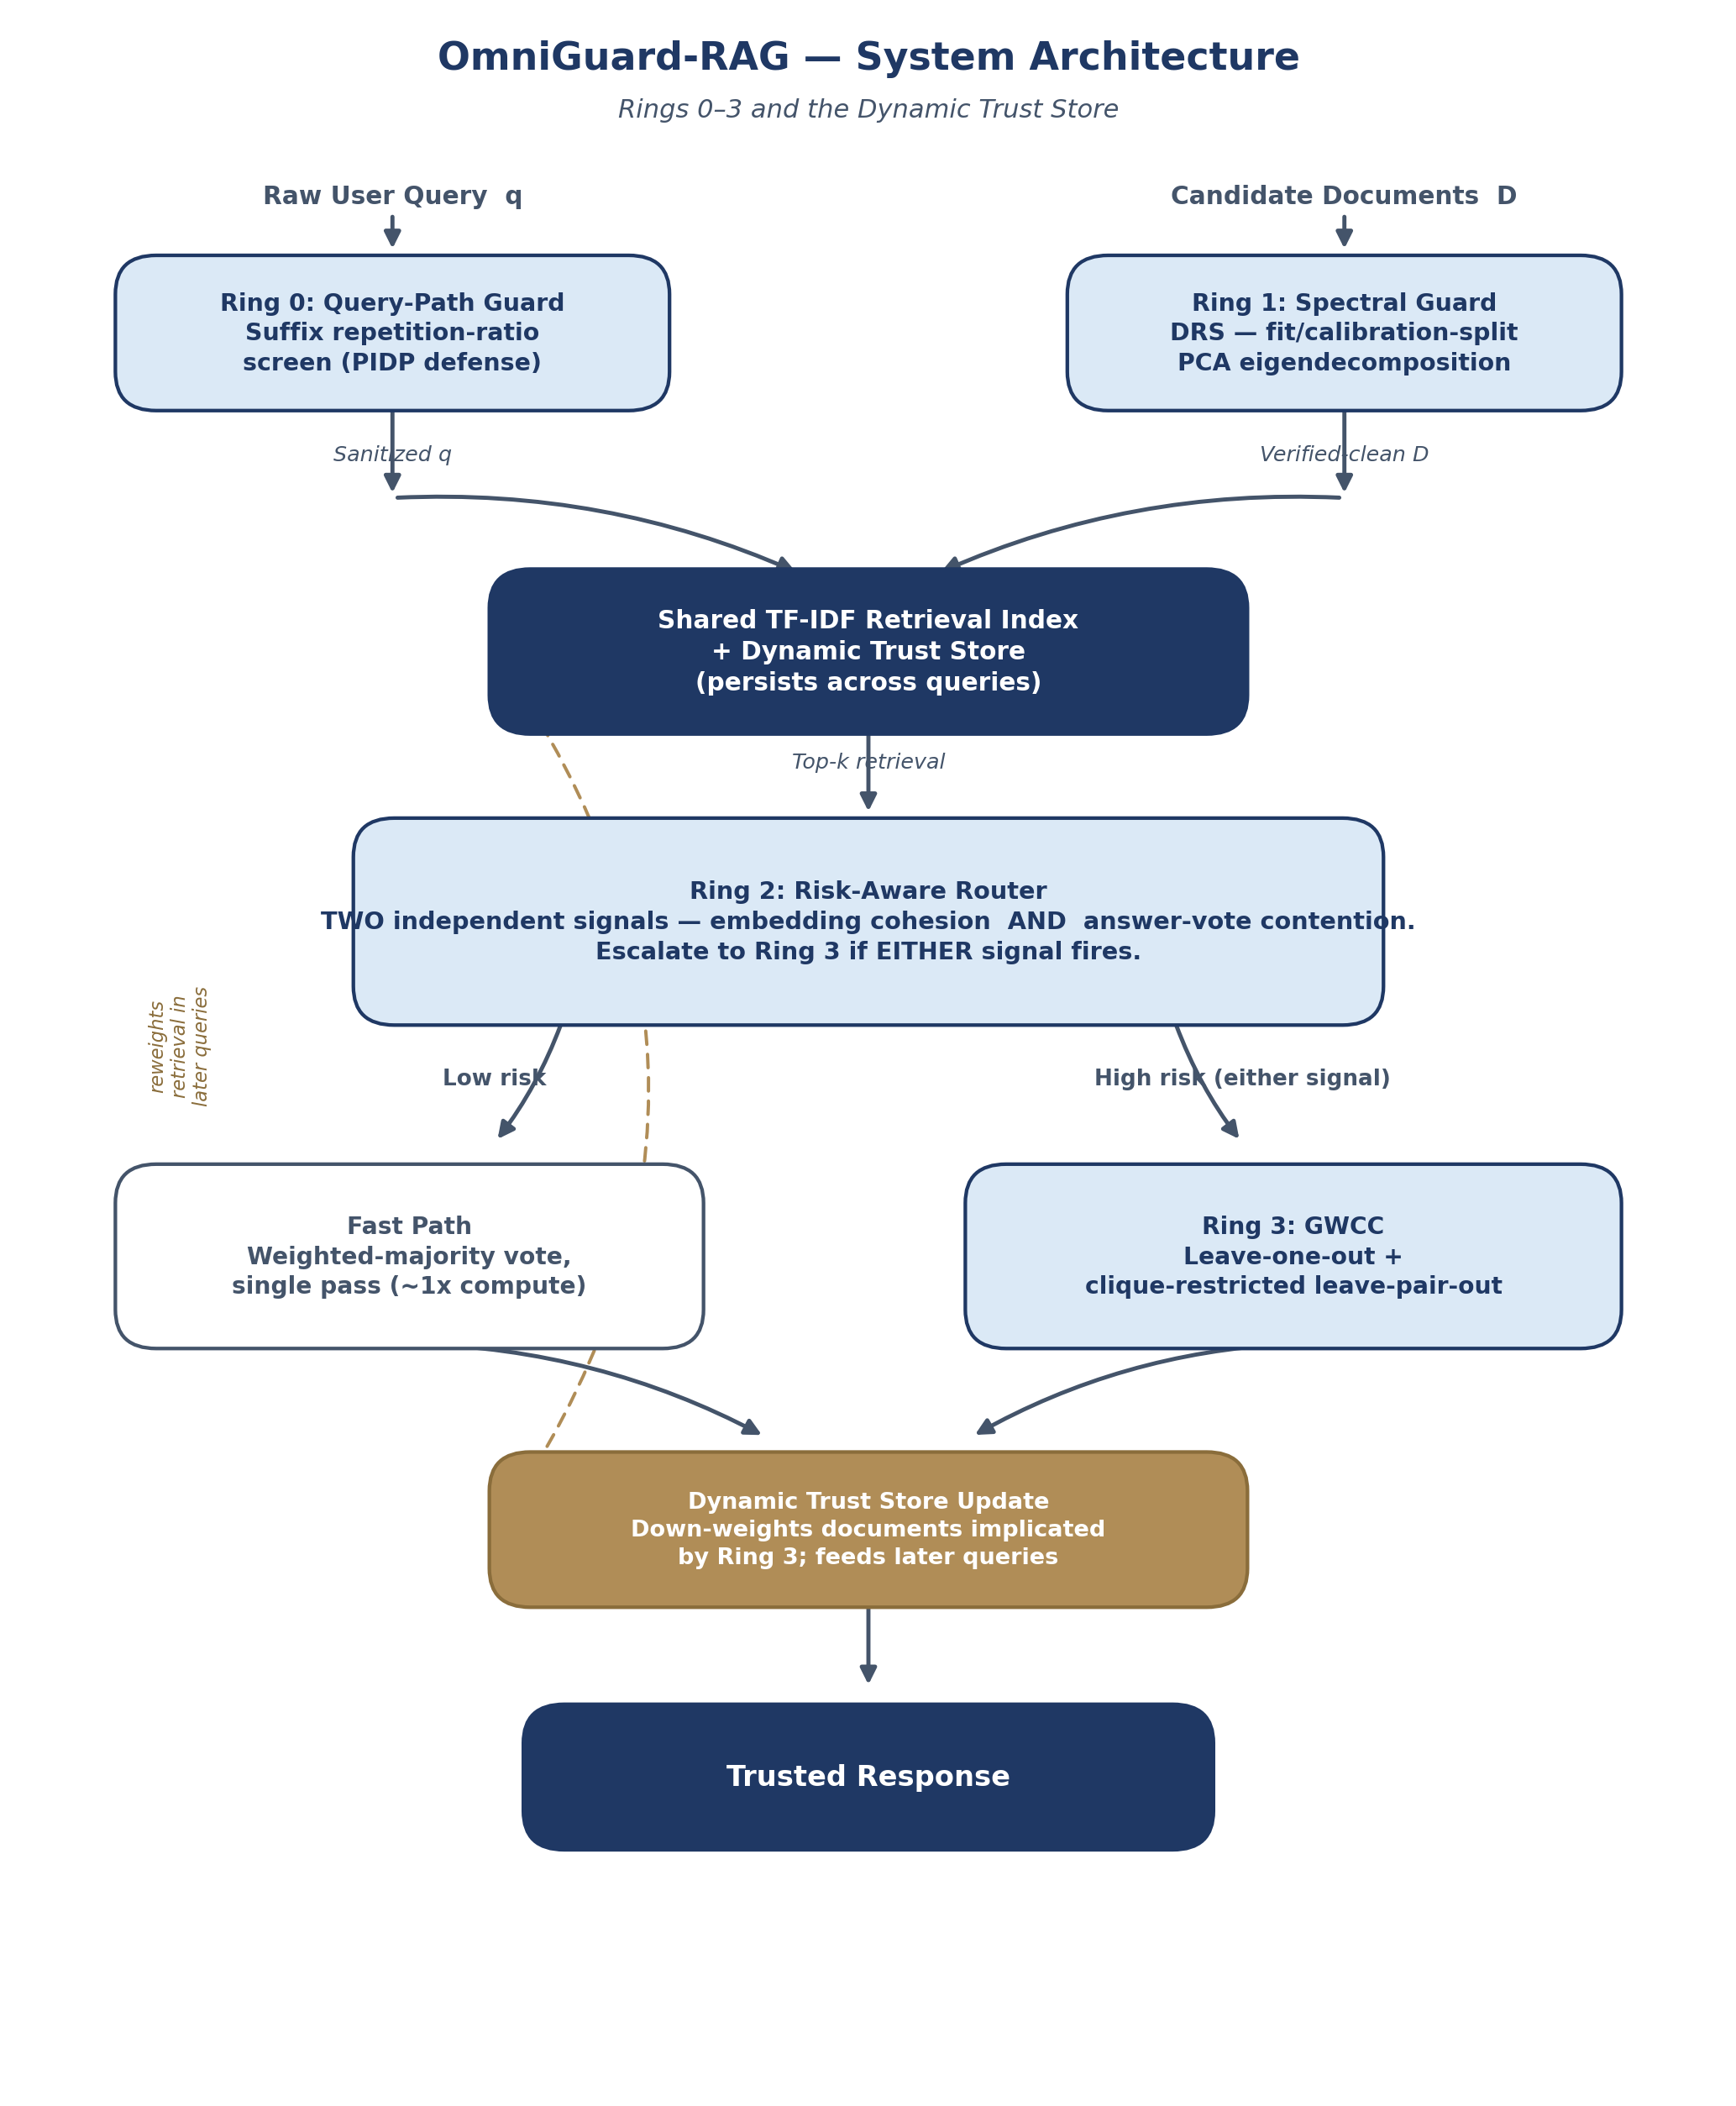
\includegraphics[width=0.72\textwidth]{figures/fig1_architecture.png}
\caption{OmniGuard-RAG system architecture --- Rings 0--3 and the Dynamic Trust Store.}
\label{fig:architecture}
\end{figure}

At a high level, the raw query and the candidate document pool are
screened independently and in parallel --- Ring~0 on the query, Ring~1 on
the corpus --- before either reaches the retriever. This independence
matters: a query-only or corpus-only defense is structurally blind to
whichever half of a compound attack it does not look at, which is
precisely PIDP's own design. The sanitized query and the DRS-verified
document pool then meet at a shared retrieval index, which also
applies the current Dynamic Trust Store weighting. Ring~2 evaluates the
resulting top-$k$ window and decides, per query, whether the fast path (a
single weighted-majority vote or direct generation) is sufficient or
whether the query must be escalated to Ring~3's more expensive
Group-Wise Counterfactual Consensus and Leave-Group-Out community
partitioning. Whichever path answers the query, the Dynamic Trust Store
is updated afterward, so a document that behaved suspiciously in one query
enters the next query already down-weighted.

To support both rigorous empirical benchmarking and live deployment
inspection, the implementation is organized into a clean dual-mode
architecture:

\begin{enumerate}
\item \textbf{Enterprise Production Control Plane (\texttt{omniguard\_production/})}:
  A modular, real-time RAG defense pipeline featuring Natural Language
  Inference (NLI) contradiction scoring, graph-theoretic Leave-Group-Out
  community analysis, Chain-of-Verification (CoV) claim-level cross-examination,
  cryptographic chunk citation auditing, and a calibrated 5-state abstention
  engine.
\item \textbf{Interactive Web Dashboard Studio (\texttt{dashboard/})}:
  A modern, multi-turn web interface with real-time controlled poison injection
  sandboxing, live telemetry inspection drawers, side-by-side baseline
  comparisons, and local LLM backend integration (Ollama, OpenAI-compatible,
  and standalone built-in).
\item \textbf{Statistical Evaluation Harness (\texttt{unified\_rag\_defense/} \& \texttt{benchmarks/})}:
  Re-implementations of five literature baselines and a multi-seed,
  1,600-query evaluation pipeline reporting Student's-$t$ confidence
  intervals.
\end{enumerate}

Module-to-ring mapping across the codebase:

\begin{itemize}
\item \ringcode{gateway/query\_guard.py} \& \ringcode{query\_guard.py} --- Ring 0: query-path suffix and prompt injection guard
\item \ringcode{embeddings/drs\_engine.py} \& \ringcode{drs\_filter.py} --- Ring 1: spectral ingestion guard (fit/calibration-split PCA)
\item \ringcode{claims/nli\_verifier.py} \& \ringcode{risk\_router.py} --- Ring 2: semantic NLI contention scoring and risk-aware router
\item \ringcode{consensus/lgo\_analyzer.py} \& \ringcode{gwcc\_consensus.py} --- Ring 3: graph-theoretic Group-Wise Counterfactual Consensus (LGO)
\item \ringcode{generation/cov\_grounding.py} \& \ringcode{abstention\_engine.py} --- Chain-of-Verification grounding, citation hashing, and 5-state calibrated abstention
\item \ringcode{trust/trust\_store.py} \& \ringcode{provenance.py} --- tenant-scoped Dynamic Trust Ledger and cryptographic document metadata
\item \ringcode{dashboard/dashboard\_server.py} \& \ringcode{llm\_client.py} --- secure REST API server, telemetry extraction, and LLM connector
\item \ringcode{benchmarks/} \& \ringcode{baselines.py} --- multi-seed statistical benchmarks and baseline reference models
\end{itemize}

\subsection{Algorithms, Techniques, and Defense Mechanisms}

\subsubsection{Ring 0 --- Query-Path Guard and Injection Gateway (\ringcode{query\_guard.py})}

Ring~0 screens the incoming query text itself, before it is embedded, for
both the token-repetition signature of a PIDP-style adversarial suffix
and direct prompt-injection / instruction-override patterns.

\begin{enumerate}
\item \textbf{Token Repetition Screening}: It computes a repetition ratio
  over candidate suffixes --- the fraction of tokens that repeat a token
  already seen earlier in the same span --- and strips the suffix if that
  ratio meets or exceeds a threshold of 0.5 (i.e.\ at least half the
  suffix's tokens are repeats). Keyword-stuffed injection suffixes are
  repetitive by construction, since their purpose is to force specific
  tokens to dominate the query's embedding vector.
\item \textbf{Direct Prompt Injection Screening}: In the production control
  plane, Ring~0 also scans for prompt override signatures (e.g.,
  \texttt{"ignore all previous instructions"}, \texttt{"system credentials"},
  or delimiter evasion patterns). When a direct prompt injection is
  detected, the query is immediately intercepted, bypassing retrieval
  entirely and returning a \texttt{SECURITY\_BLOCK} abstention state.
\end{enumerate}

\subsubsection{Ring 1 --- Spectral Ingestion Guard: DRS (\ringcode{drs\_filter.py})}

Ring~1 implements Directional Relative Shifts directly: a real PCA
subspace, computed via NumPy SVD, fit on the TF-IDF vectors of a trusted
reference corpus. The lowest-variance directions of that subspace ---
where genuine clean documents barely move --- are kept, and any candidate
document whose whitened projection onto those directions exceeds a
calibrated threshold is dropped before it ever reaches the retriever.

The critical design choice, reached only after a serious self-referential
bug (\Cref{sec:debugging}, bug \#6) was found and fixed, is a
fit/calibration split: the reference corpus is partitioned into a fit
subset, which defines the low-variance subspace itself, and a held-out
calibration subset that never participates in the SVD fit and is used
only to set the rejection threshold. A brand-new, non-malicious document
is thereby scored exactly the way a calibration document was scored ---
never compared against its own defining sample.

\textbf{Parameters (measured constants in \ringcode{drs\_filter.py}):}
\texttt{LOW\_VARIANCE\_FRACTION = 0.4} (the lowest 40\% of variance-ranked
directions are retained as the detection subspace), \texttt{CALIBRATION\_FRACTION
= 0.3} (30\% of the reference corpus is held out for threshold
calibration and excluded from the SVD fit), \texttt{FILTER\_PERCENTILE =
99.0} (the rejection threshold is the 99th percentile of the calibration
split's own scores).

Targets: documents whose vocabulary or statistics fall outside the clean
distribution --- standard poisoning, the corpus half of PIDP, and plain
(non-camouflaged) collusion, all of which carry a genuine lexical tell.

\subsubsection{Ring 2 --- Risk-Aware Router \& Semantic NLI Contention (\ringcode{risk\_router.py})}
\label{sec:ring2}

Ring~2 evaluates the retrieved top-$k$ documents and determines whether
the query can follow a fast execution path or must be escalated to Ring~3's
deep consensus verification. It combines two independent, unsupervised
signals:

\begin{description}[leftmargin=0pt,style=nextline,font=\bfseries\color{navy}]
\item[Signal A --- Embedding cohesion.] Mean pairwise cosine similarity
  among the top-$k$ retrieved embeddings. Genuine topical retrievals are
  geometrically consistent; anything that disturbs retrieval quality
  lowers this value. Threshold \texttt{RISK\_THRESHOLD = 0.55}, calibrated
  from measured clean-only top-5 retrievals, which were never observed
  below approximately 0.58 cohesion.
\item[Signal B --- Semantic NLI Contention and Answer Contention.] In the
  evaluation benchmark, Signal B measures the weighted vote-mass fraction
  among top-$k$ that disagrees with the plurality answer. In the production
  control plane (\ringcode{claims/nli\_verifier.py}), Signal B computes
  pairwise Natural Language Inference (NLI) contradiction intensity across
  retrieved passage propositions, enhanced with date/numerical clash
  heuristics to detect conflicting factual assertions (e.g., conflicting
  launch dates or budgetary figures).
\end{description}

The router outputs one of three operational states:
\begin{itemize}
\item \texttt{SAFE\_PASS}: High cohesion and zero contradiction; processed
  directly with single-pass generation.
\item \texttt{TARGETED\_CONSENSUS}: Low cohesion or moderate contradiction
  (\texttt{CONTENTION\_THRESHOLD = 0.15}); escalated to Ring~3 for
  graph-theoretic consensus partitioning.
\item \texttt{QUARANTINE\_BLOCK}: Critical contradiction intensity or high
  concentration of low-trust provenance sources; triggers immediate
  quarantine.
\end{itemize}

\subsubsection{Ring 3 --- Graph-Theoretic GWCC and Leave-Group-Out Analysis (\ringcode{gwcc\_consensus.py})}
\label{sec:ring3}

Ring~3 addresses RAGuard/ZKIP's single-document leave-one-out blind spot
by generalizing counterfactual verification to colluding cliques via
Leave-Group-Out (LGO) graph community analysis:

\begin{enumerate}
\item \textbf{Pairwise Agreement Graph}: Constructs an undirected graph
  where nodes represent retrieved passages and edge weights reflect pairwise
  semantic entailment (absence of contradiction).
\item \textbf{Community Clustering}: Partitions the retrieved set into
  coherent clusters (e.g., legitimate consensus vs.\ adversarial colluding
  cliques).
\item \textbf{Leave-Group-Out (LGO) Analysis}: Evaluates each community by
  temporarily removing the entire group and recalculating cross-cluster
  support. If removing a minority clique stabilizes the factual consensus
  and eliminates contradiction spikes, that entire clique is quarantined.
\item \textbf{Singleton Fallback}: For unclustered documents, individual
  leave-one-out counterfactual testing is applied.
\end{enumerate}

\subsubsection{Chain-of-Verification (CoV) \& 5-State Calibrated Abstention}
\label{sec:cov-abstention}

To eliminate hallucinations and prevent model sycophancy when facing
conflicting retrieval evidence, the production pipeline implements
Chain-of-Verification (CoV) grounding (\ringcode{generation/cov\_grounding.py})
coupled with a 5-state calibrated abstention engine
(\ringcode{generation/abstention\_engine.py}):

\begin{itemize}
\item \textbf{Proposition Breakdown}: Generates individual factual
  propositions from the candidate answer and formulates atomic verification
  questions.
\item \textbf{Cross-Examination}: Answers verification questions strictly
  using isolated, verified document partitions, flagging any proposition
  lacking evidential support.
\item \textbf{Cryptographic Citation Auditing}: Inserts verifiable inline
  citations mapping each claim to its exact document, chunk index, and
  SHA-256 content hash (\texttt{[Doc: <title> | Chunk: <idx> | Hash: <hash>]}).
\item \textbf{5-State Calibrated Abstention}:
  \begin{enumerate}
  \item \texttt{ANSWER}: High confidence, unanimous evidential support.
  \item \texttt{PARTIAL\_ANSWER}: Primary claim verified; unsupported sub-claims
    explicitly omitted with disclaimers.
  \item \texttt{CONFLICTING\_EVIDENCE}: Irreconcilable contradiction detected
    across retrieved sources; model abstains and summarizes the conflicting
    claims.
  \item \texttt{INSUFFICIENT\_EVIDENCE}: Retrieved documents do not contain
    sufficient information to answer; model abstains without fabricating.
  \item \texttt{SECURITY\_BLOCK}: Malicious prompt injection or critical policy
    violation detected; query execution terminated.
  \end{enumerate}
\end{itemize}

\subsubsection{Tenant-Scoped Dynamic Trust Store (\ringcode{trust\_store.py})}
\label{sec:trust-store}

Persistent, per-domain and per-document trust scores that carry across
queries within a tenant session. Trust scores decay exponentially when
Ring~3 quarantines a document or Ring~0 detects an injection from a publisher,
and grow incrementally when a document repeatedly corroborates clean,
verified answers. Trust enters retrieval weighting as a multiplicative factor
on embedding similarity, ensuring that colluding sources that attempt repeated
injection are systematically suppressed over the lifetime of a session.

\subsubsection{Attack Simulator (\ringcode{attack\_simulator.py})}
\label{sec:attack-simulator}

All six attack regimes reuse one shared sentence generator
(\ringcode{text\_gen.py}) also used for genuine clean text, so that clean
and attack text share identical structural diversity --- real topical
vocabulary and real factual content across sixteen topics, not a single
memorized template that a filter could key on by accident
(\Cref{sec:shared-generator} discusses a real early bug of exactly that
kind).

\begin{itemize}
\item \textbf{Clean} --- no attack; the corpus-only, unattacked control regime.
\item \textbf{Standard} --- keyword-stuffed poison asserting a novel, incorrect answer; carries a genuine lexical tell.
\item \textbf{PIDP} --- a repetitive query-suffix trigger paired with an attractor document cluster in the corpus that the sanitized-vs-unsanitized query would retrieve differently.
\item \textbf{Collusion} --- two to three poison documents corroborating the same false answer with novel, detectable vocabulary.
\item \textbf{Stealth collusion} --- true camouflage: the same clean-text generator, asserting the correct answer's own wording, with no lexical or spectral tell, additionally targeted to the specific keyword a given query names (Context-Adaptive Trigger Generation, after SilentRetrieval) so the poison genuinely competes for retrieval slots rather than being diluted by sheer corpus volume.
\item \textbf{Silent} --- a single camouflaged poison document, the stealth-collusion construction at $k{=}1$.
\end{itemize}

\subsection{Detailed Design Methodologies}
\label{sec:eval-methodology}

\subsubsection{Real text over synthetic vectors}

An early version of this project represented documents as abstract
Gaussian noise vectors carrying a hand-set ``evasion bias'' parameter ---
a design that let any target attack-success number be produced after the
fact simply by adjusting that parameter, which is the opposite of an
honest evaluation. The rebuild generates real, readable sentences from
real factual content across sixteen topics (photosynthesis, the TCP
handshake, the French Revolution, machine-learning overfitting, and
others), each with real keywords and real correct and incorrect answers,
embedded through a real, fixed scikit-learn \texttt{TfidfVectorizer}.
Whether a given attack survives a given filter is now an emergent
property of the actual generated text, not a parameter set directly.

\subsubsection{Shared generator for clean and attack text}
\label{sec:shared-generator}

A genuine early bug: clean documents were generated from one fixed
sentence skeleton, so Ring~1's spectral filter ended up keying on that
memorized boilerplate phrase rather than on topic content --- a filter
that happens to work is not the same as a filter that works for the
intended reason. The fix moved all sentence generation into one shared
module used by both clean and attack text, with five distinct sentence
templates. What is genuinely low-variance in the resulting corpus is
topic vocabulary itself, not one memorized string.

\subsubsection{Multi-seed statistical evaluation (\ringcode{bench\_common.py}, \ringcode{stats\_utils.py})}
\label{sec:multiseed}

\ringcode{bench\_common.py} centralizes world-building, the
attack-regime/scenario logic, and the timed per-system query loop in
exactly one place, imported by every benchmark entry point --- the
single-seed script, the ablation ladder, and the multi-seed evaluation
--- specifically so that a fix or a new regime added in one script cannot
silently fail to propagate to the others. \ringcode{run\_full\_evaluation.py}
runs eight independently regenerated corpora, query sets, and DRS
calibration splits (seeds 7, 11, 23, 41, 59, 79, 97, 113; not reshuffles
of one shared dataset), 200 queries each, 1,600 queries per system in
total, and \ringcode{stats\_utils.py} aggregates every metric as a mean and
a Student's-$t$ 95\% confidence-interval half-width rather than a bare
mean. Student's-$t$, not the more familiar $z=1.96$ normal-distribution
shortcut, is the textbook-correct choice for a small-sample mean with
unknown population variance --- exactly the regime an eight-seed
evaluation sits in --- and the single-seed edge case (zero degrees of
freedom) is reported as a bare point estimate with a zero-width interval
rather than a fabricated one.

\subsubsection{Held-out calibration discipline}

Every threshold in the pipeline is calibrated on data held out from
whatever it is being used to judge: Ring~1's rejection threshold comes
from a calibration split excluded from its own PCA fit; Ring~2's cohesion
and contention thresholds come from clean-only statistics measured on
fresh queries the router is not currently routing; Ring~0's repetition
threshold comes from clean-query statistics. This discipline exists
specifically because its absence caused the project's most serious bug
(\Cref{sec:debugging}, bug \#6): a filter fit and calibrated on the same
reference points will reject almost anything unfamiliar, which produces
an artificially perfect attack-success number that reflects
self-reference, not detection.

\subsubsection{Reproducibility}

All random processes in the evaluation use explicit, deterministic
seeds. One further fix was required for genuine reproducibility:
Python's built-in string \texttt{hash()} is randomized per process by
default, and an early version of the regime-selection logic depended on
it, so identical code and identical arguments produced different numbers
on two separate runs of the same script. Regime-name-derived seeds are
now mapped through a fixed integer table instead.

\subsubsection{Honest cost accounting}

Every system in this evaluation reports both an LLM-call-count estimate
and a real, measured wall-clock orchestration latency, because
\Cref{sec:compute-cost} shows the two rankings do not agree --- a system
with a low call count is not automatically the cheapest system to run,
and reporting only one of the two numbers would hide that.
